\raggedright

\section{I/O Ports}

Ports werden durch 8 Bit Register konfiguriert.

Der ATmega328p hat insgesamt 3 Portbänke (B, C und D).

Ports können auch mehrfach belegt sein!


\subsection{Data Direction Register}

Die Data Direction Register der jeweiligen Ports legen die Richtung fest.

0 = Input (Default), 1 = Output

\vspace{2em}
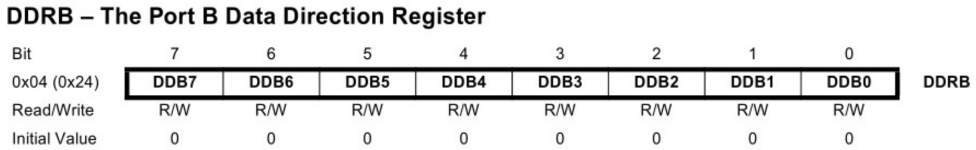
\includegraphics[scale=0.5]{DDRB.png}
\vspace{2em}

